\documentclass{article}

\usepackage[font=small]{caption}

\usepackage{nips_2016} 
\usepackage{xspace}
\usepackage{setspace}

\usepackage[utf8]{inputenc} % allow utf-8 input
\usepackage[T1]{fontenc}    % use 8-bit T1 fonts
\usepackage{hyperref}       % hyperlinks
\usepackage{url}            % simple URL typesetting
\usepackage{booktabs}       % professional-quality tables
\usepackage{amsfonts}       % blackboard math symbols
\usepackage{nicefrac}       % compact symbols for 1/2, etc.
\usepackage{microtype}      % microtypography
\usepackage{graphicx} % more modern
%\usepackage{subfigure} 
\usepackage{subcaption}
% For algorithms
\usepackage{algorithm}
\usepackage{algorithmic}
\usepackage{wrapfig}
\usepackage[all]{xy}

% Packages hyperref and algorithmic misbehave sometimes.  We can fix
% this with the following command.
%\newcommand{\theHalgorithm}{\arabic{algorithm}}

% Employ the following version of the ``usepackage'' statement for
% submitting the draft version of the paper for review.  This will set
% the note in the first column to ``Under review.  Do not distribute.''
\usepackage{amsmath,amsfonts,amssymb}
\usepackage{dsfont}
\usepackage{booktabs}
\usepackage{relsize}
\usepackage{siunitx}

\newcommand{\xsb}{\mathbf{\hat{x}}_{1,\ldots,B}}
\newcommand{\ysb}{\hat{y}_{1,\ldots,B}}
\newcommand{\xub}{\mathbf{x}_{1,\ldots,B}}


\newcommand{\xsj}{\mathbf{\hat{x}}_j}
\newcommand{\xsi}{\mathbf{\hat{x}}_i}
\newcommand{\ysi}{\hat{y}_i}
\newcommand{\ysj}{\hat{y}_j}

\newcommand{\xuj}{\mathbf{x}_j}
\newcommand{\xui}{\mathbf{x}_i}
\newcommand{\yui}{y_i}
\newcommand{\yuj}{y_j}
\newcommand{\sw}{s_{ \textsc{\relsize{-2}{\textsl{W}}} }}

\newcommand*{\eg}{e.g.\@\xspace}

\newcommand\at[2]{\left.#1\right|_{#2}}

% Employ this version of the ``usepackage'' statement after the paper has
% been accepted, when creating the final version.  This will set the
% note in the first column to ``Proceedings of the...''
%\usepackage[accepted]{icml2016}


% The \icmltitle you define below is probably too long as a header.
% Therefore, a short form for the running title is supplied here:

%\title{Consistent Transduction for Unsupervised Domain Adaptation}
\title{Learning Transferrable Representations for Unsupervised Domain Adaptation \\ -  \\Supplementary Material}

\author{
  David S.~Hippocampus\thanks{Use footnote for providing further
    information about author (webpage, alternative
    address)---\emph{not} for acknowledging funding agencies.} \\
  Department of Computer Science\\
  Cranberry-Lemon University\\
  Pittsburgh, PA 15213 \\
  \texttt{hippo@cs.cranberry-lemon.edu} \\
  %% examples of more authors
  %% \And
  %% Coauthor \\
  %% Affiliation \\
  %% Address \\
  %% \texttt{email} \\
  %% \AND
  %% Coauthor \\
  %% Affiliation \\
  %% Address \\
  %% \texttt{email} \\
  %% \And
  %% Coauthor \\
  %% Affiliation \\
  %% Address \\
  %% \texttt{email} \\
  %% \And
  %% Coauthor \\
  %% Affiliation \\
  %% Address \\
  %% \texttt{email} \\
}

\begin{document} 

\maketitle

\begin{abstract} 
In this supplementary material, we study the sensitivity of the parameter $M$ and give details on the computation of sub-gradient of the loss function with respect to feature weights $\theta_c,\theta_s,\theta_t$. Cost of the reject option $\gamma$ is function of the parameter $M$ and we show that, it is possible to obtain high accuracy over a wide range of $M$ values.
\end{abstract} 

\section{Sensitivity Analysis of $M$}
As we explained in the main paper, we use the following update function to control the reject cost during training; $\gamma = 0.1 + \frac{\#epoch -1}{M}$. In order to analyze the sensitivity of our algorithm on $M$, we swept the scaling factor ($M$) between 0 and 160 in the SVHN$\rightarrow$MNIST experiment. We computed accuracy for each value of $M$ after the adaptation is completed. We display the resulting accuracy vs $M$ plot in Figure~\ref{sens}.



\begin{figure}[h]
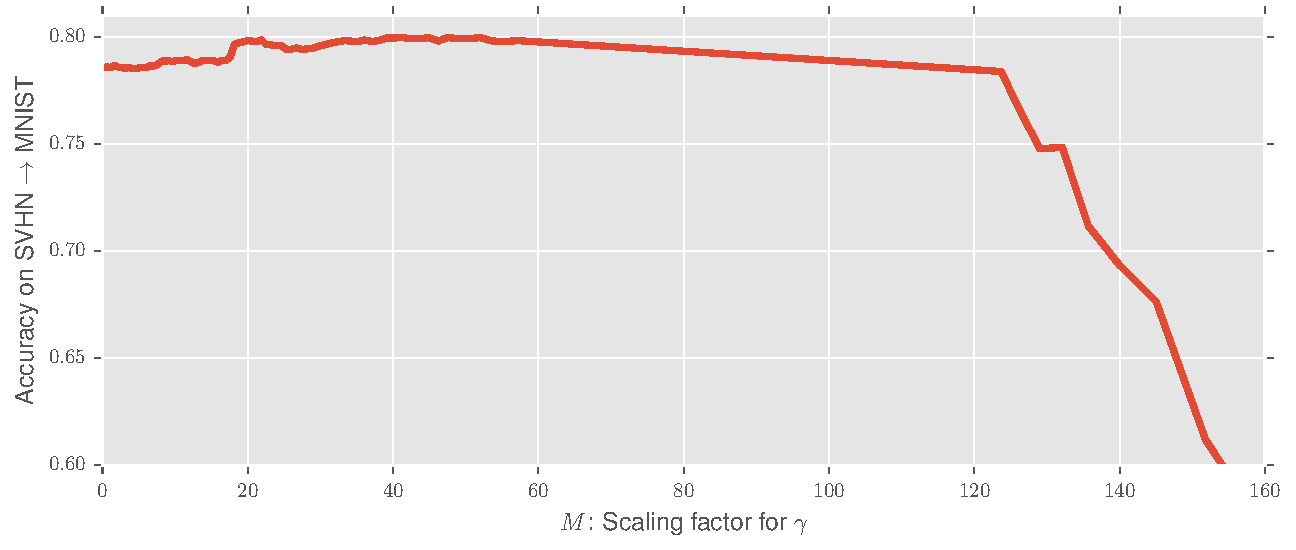
\includegraphics[width=\textwidth]{a.pdf}
\caption{Effect of reject cost -$\gamma$- on the accuracy. Please note that there is large range of $M$ values yielding high accuracy. Hence, our model is not sensitive to the $M$ parameter.}
\label{sens}
\end{figure}

Figure~\ref{sens} shows that there is a large range of values for $M$ which results in high accuracy transduction. Moreover, for very-large values of $M$, the reject cost $\gamma$ will almost always be low during the training preventing transduction algorithm to make any prediction other than reject. Hence, we expect this set-up to perform similarly to \textbf{source only} baseline since adaptation is not possible when all labels are reject. Whereas, for very-small values of $M$, the reject cost $\gamma$ will immediately be very-large and our transduction method will not be able to predict reject at all. Hence, we expect this setup to perform similarly to \textbf{no reject} baseline. Indeed, we see this asymptotic behavior and the extreme values of the plot is compatible with numbers in Table~2 of the main paper.

\section{Sub-gradients of the loss function for adaptation} 
We need the explicit form of feature functions to compute the sub-gradients. With a slight abuse of notation, we define the following functions $\Phi_s(\cdot) = \phi_s (\phi_c(\cdot))$ and $\Phi_t(\cdot) = \phi_t (\phi_c(\cdot))$ such that $\phi_s$, $\phi_t$ and $\phi_c$ are functions of $\theta_s$, $\theta_t$ and $\theta_c$ respectively.

Using these terms, we can re-write the loss function from (main paper 3) as;
\begin{equation}
loss =  \sum_{i \in [N^s]} [\phi_{s}(\phi_{c}(\xsi))^\intercal \phi_{t}(\phi_{c}(\mathbf{x}_{i^-})) -\phi_{s}(\phi_{c}(\xsi))^\intercal \phi_{t}(\phi_{c}(\mathbf{x}_{i^+})) + \alpha]_{+}
\end{equation}

The sub-gradients can then further be computed as;

{\scriptsize
\begin{equation}
\begin{aligned}
\frac{\partial loss}{\partial \theta_s} = &\sum_{i \in [N^s]} \mathds{1}(\Phi_s(\xsi)^\intercal \Phi_t(\mathbf{x}_{i^+}) - \Phi_s(\xsi)^\intercal \Phi_t(\mathbf{x}_{i^-}) < \alpha) \left[ \at{\frac{\partial \phi_s}{\partial \theta_s}}{\phi_c(\xsi)} \left(\Phi_t(\mathbf{x}_{i^-}) -  \Phi_t(\mathbf{x}_{i^+})\right) \right] \\
\frac{\partial loss}{\partial \theta_t} = &\sum_{i \in [N^s]} \mathds{1}(\Phi_s(\xsi)^\intercal \Phi_t(\mathbf{x}_{i^+}) - \Phi_s(\xsi)^\intercal \Phi_t(\mathbf{x}_{i^-}) < \alpha) \left[ \left( \at{\frac{\partial \phi_t  } {\partial \theta_t}}{\phi_c(\mathbf{x}_{i^-})}  - \at{\frac{\partial \phi_t} {\partial \theta_t}}{\phi_c(\mathbf{x}_{i^+})}  \right)  \Phi_s(\xsi) \right] \\
\frac{\partial loss}{\partial \theta_c} = &\sum_{i \in [N^s]} \mathds{1}(\Phi_s(\xsi)^\intercal \Phi_t(\mathbf{x}_{i^+}) - \Phi_s(\xsi)^\intercal \Phi_t(\mathbf{x}_{i^-}) < \alpha) \times \\
&\left[ \at{\frac{\partial \phi_s}{\partial \phi_c}}{\phi_c(\xsi)} \at{\frac{\partial \phi_c}{\theta_c}}{\xsi} \left(\Phi_t(\mathbf{x}_{i^-}) - \Phi_t(\mathbf{x}_{i^+})\right)  \right.  + \left.  \left(\at{\frac{\partial \phi_t}{\partial \phi_c}}{\phi_c(\mathbf{x}_{i^-})} \at{\frac{\partial \phi_c}{\theta_c}}{\mathbf{x}_{i^-}} - \at{\frac{\partial \phi_t}{\partial \phi_c}}{\phi_c(\mathbf{x}_{i^+})} \at{\frac{\partial \phi_c}{\theta_c}}{\mathbf{x}_{i^+}}\right) \Phi_s (\xsi) \right]
\end{aligned}
\end{equation}
}



\clearpage
\setlength{\bibsep}{2pt plus 0.25ex}
{\small
\bibliography{domain_transduction_s}
\bibliographystyle{abbrv}
}
\end{document} 